\documentclass[10pt,a4paper]{article}
\usepackage[T1]{fontenc}
\usepackage[utf8]{inputenc}
\usepackage{mathpazo}
\usepackage[margin=24mm]{geometry}
\usepackage{amsmath}
\usepackage{booktabs}
\usepackage{longtable}
\usepackage{graphicx}
\usepackage[obeyspaces]{url}
\renewcommand{\UrlBreaks}{\do\_\do\/\do\[\do\]\do\.\do\-\do\,}
\setlength{\parindent}{0pt}
\setlength{\parskip}{5pt}
\begin{document}

\begin{center}
{\LARGE DIPESH --- test report}\\[6pt]
DIPESH --- Detection and Imaging of Pbar Events, Spots and Hits\\[4pt]
version 1.0.0\\
report written 2026-10-08
\end{center}

\section{Summary}
256 tests: 256 passed, 0 failed, 0 skipped. pytest reported: 256 passed in 100.99s (0:01:40).
\begin{center}
\begin{tabular}{lrrrrr}
\toprule
package & tests & passed & failed & skipped & not run \\
\midrule
Single-image analysis & 40 & 40 & 0 & 0 & 0 \\
Spot features & 83 & 83 & 0 & 0 & 0 \\
Clustering and recognition & 14 & 14 & 0 & 0 & 0 \\
Results & 19 & 19 & 0 & 0 & 0 \\
Pickup & 23 & 23 & 0 & 0 & 0 \\
Graphical interface & 52 & 52 & 0 & 0 & 0 \\
Whole program & 25 & 25 & 0 & 0 & 0 \\
\midrule
all & 256 & 256 & 0 & 0 & 0 \\
\bottomrule
\end{tabular}
\end{center}
Software: Python 3.11.0, numpy 2.4.6, OpenCV 5.0.0, scipy 1.17.1, matplotlib 3.11.2, PySide6 6.12.0, pyqtgraph 0.14.0; Windows 10, Intel64 Family 6 Model 191 Stepping 2, GenuineIntel.

\section{The six reference frames}
Every count, every per-spot value and every per-image value of the six reference frames (synthetic, written by \path{tests/reference/make_frames.py}) is compared with \path{tests/reference/golden.json}. Counts, integers and booleans must be equal; decimal values must agree to $10^{-12}$ relative.
\begin{center}
\begin{tabular}{lrrrrrrl}
\toprule
frame & \multicolumn{2}{c}{count} & values & outside & last-bit & largest rel.\ diff. & field \\
 & ref. & now & & tolerance & only & & \\
\midrule
1 & 23 & 23 & 306 & 0 & 0 & 0 & - \\
2 & 44 & 44 & 579 & 0 & 0 & 0 & - \\
3 & 34 & 34 & 449 & 0 & 0 & 0 & - \\
4 & 27 & 27 & 358 & 0 & 0 & 0 & - \\
5 & 3 & 3 & 46 & 0 & 0 & 0 & - \\
6 & 7 & 7 & 98 & 0 & 0 & 0 & - \\
\bottomrule
\end{tabular}
\end{center}
{\small Frames: 1 = \path{frame_1.tiff}; 2 = \path{frame_2.tiff}; 3 = \path{frame_3.tiff}; 4 = \path{frame_4.tiff}; 5 = \path{frame_5.tiff}; 6 = \path{frame_6.tiff}.}


\section{Reading the data}
\begin{longtable}{@{}p{0.86\textwidth}r@{}}
\toprule
test & result \\
\midrule
\endhead
scan handles run folders loose images and files & passed \\
scan of a single run folder gives one item & passed \\
scan of nothing useful is empty & passed \\
run folders are sorted by run number & passed \\
the tiff is found one folder down & passed \\
an image is read at its own bit depth & passed \\
batman parameters are read & passed \\
a missing or broken batman gives no parameters & passed \\
\bottomrule
\end{longtable}

\section{Preprocessing: hot pixels, bit depth, background}
A pixel is hot when $I > \mathrm{med}_{3\times3}(I) + \delta$ and takes that median. The image is scaled by the camera bit depth, $I \to 255\,I/F$, with $F$ the smallest of 255, 1023, 4095, 65535 that holds the maximum. The background is $B = (G * IM)/(G * M)$, $G$ a Gaussian blur and $M$ the mask of pixels with $I - G * I < n\,\sigma$, $\sigma = 1.4826\,\mathrm{MAD}$.

\begin{longtable}{@{}p{0.86\textwidth}r@{}}
\toprule
test & result \\
\midrule
\endhead
hot pixels are removed not counted & passed \\
a hot pixel is replaced by its 3x3 median\newline{\small\itshape A pixel more than hotpix\_delta above the median of its 3x3 neighbourhood takes that median.} & passed \\
hot pixel delta zero switches the correction off & passed \\
the peak of a real spot is not a hot pixel\newline{\small\itshape A spot of sigma 1.5 px: the peak is 22 \% above its neighbours, far less than hotpix\_delta.} & passed \\
hot pixel delta scales with the bit depth\newline{\small\itshape On a 12-bit image the same delta means 60 * 4095 / 255 counts.} & passed \\
normalisation is by bit depth not content & passed \\
the full scale is the smallest bit depth that holds the maximum\newline{\small\itshape out = in * 255 / full\_scale, full\_scale in (255, 1023, 4095, 65535).} & passed (8/8) \\
an 8 bit image is not rescaled & passed \\
the masked background does not rise under a bright spot\newline{\small\itshape A plain 51 px blur lifts the baseline under a spot of A = 200, sigma = 2.2 by more than 5 counts; the masked second pass stays within one count of the true offset (only the faint tail below the mask level still leaks in).} & passed \\
a flat image has itself as background & passed \\
the noise estimate is the gaussian sigma\newline{\small\itshape sigma = 1.4826 * MAD recovers the sigma of Gaussian noise (2 \%).} & passed \\
prepare returns a non negative image on the 0 255 scale & passed \\
\bottomrule
\end{longtable}

\section{Detection}
With $D = \max(I - B, 0)$, a pixel is a candidate when it is the maximum of its neighbourhood, $D > T$, $S_5 > S_{\min}$ and $S_5/D > s_{\min}$, where $S_5$ is the $5\times5$ sum and $T = \max(T_{\mathrm{abs}},\, n\,\sigma)$. Candidates are taken brightest first; each removes the others within $d_{\min}$.

\begin{longtable}{@{}p{0.86\textwidth}r@{}}
\toprule
test & result \\
\midrule
\endhead
finds every planted spot & passed \\
empty frame has no spots & passed \\
raising the threshold never adds spots & passed \\
photometry does not change the count & passed \\
two peaks closer than min dist are one particle\newline{\small\itshape Peaks 8 px apart with min\_dist = 12 -\textgreater{} count 1; with min\_dist = 6 -\textgreater{} 2.} & passed \\
two peaks further than min dist are two particles\newline{\small\itshape Peaks 20 px apart with min\_dist = 12 -\textgreater{} count 2.} & passed \\
a flat topped spot is counted once\newline{\small\itshape A saturated spot has several pixels at the maximum; NMS keeps one.} & passed \\
the adaptive threshold is the larger of the two\newline{\small\itshape thresh = max(abs\_thresh, n\_sigma * noise); abs\_thresh alone when adaptive is off.} & passed \\
\bottomrule
\end{longtable}

\section{Aperture}
$L(r) = \sum_{\rho \le r} (D - b)$ is summed in growing discs. The aperture stops at the first $r$ with $L(r) - L(r-1) < f\,L(r-1)$ ($f$ = plateau\_frac $= 0.02$), or at spot\_max\_radius.

\begin{center}
\begin{tabular}{lrrrrl}
\toprule
case & true & measured & absolute error & tolerance & \\
\midrule
sigma = 1.5 px & 6 & 6 & 0 & 1 & ok \\
sigma = 2 px & 7 & 7 & 0 & 1 & ok \\
sigma = 3 px & 9 & 10 & 1 & 1 & ok \\
sigma = 6 px & 12 & 12 & 0 & 1 & ok \\
\bottomrule
\end{tabular}
\end{center}
\noindent{\small Radius used, against the rule applied to a continuous Gaussian (absolute error, px).}

\begin{longtable}{@{}p{0.86\textwidth}r@{}}
\toprule
test & result \\
\midrule
\endhead
the radius grows with the spot size\newline{\small\itshape R(sigma) is non-decreasing, and larger for sigma = 3 than for 1.5.} & passed \\
the radius is where a ring adds less than plateau frac\newline{\small\itshape R = first r with L(r) - L(r-1) \textless{} 0.02 L(r-1), L(r) = 1 - exp(-r\textasciicircum{}2 / 2 sigma\textasciicircum{}2); within 1 px.} & passed (4/4) \\
the radius stops at spot max radius\newline{\small\itshape A spot of sigma = 6 px never plateaus within 12 px: R = spot\_max\_radius.} & passed (3/3) \\
a larger plateau frac never gives a larger radius\newline{\small\itshape R(plateau\_frac) is non-increasing.} & passed (3/3) \\
the centroid is the centre of the spot\newline{\small\itshape Centroid = sum(w x) / sum(w): the centre of a Gaussian placed 0.3 px right and 0.2 px down of the pixel, to 1e-3 px.} & passed \\
the local window gives the same numbers as the full frame\newline{\small\itshape The aperture mask built in the window equals the full-frame mask.} & passed \\
a spot at the image edge uses the pixels that exist & passed \\
\bottomrule
\end{longtable}

\section{Luminosity}
$L = \sum_{\rho \le R} (D - b)$. For a Gaussian spot of amplitude $A$ and width $\sigma$: $L = 2\pi A \sigma^2\,(1 - e^{-R^2/2\sigma^2})$.

\begin{center}
\begin{tabular}{lrrrrl}
\toprule
case & true & measured & relative error & tolerance & \\
\midrule
sigma = 1.5 px & 1413.72 & 1413.72 & $7.3\times10^{-8}$ & $1.0\times10^{-4}$ & ok \\
sigma = 2 px & 2513.27 & 2513.27 & $1.9\times10^{-8}$ & $1.0\times10^{-4}$ & ok \\
sigma = 3 px & 5654.87 & 5654.87 & $1.0\times10^{-7}$ & $1.0\times10^{-4}$ & ok \\
\bottomrule
\end{tabular}
\end{center}
\noindent{\small Aperture out to $6\sigma$.}

\begin{center}
\begin{tabular}{lrrrrl}
\toprule
case & true & measured & relative error & tolerance & \\
\midrule
sigma = 1.5 px, R = 6 px & 1413.72 & 1413.22 & $3.5\times10^{-4}$ & $3.0\times10^{-2}$ & ok \\
sigma = 2 px, R = 7 px & 2513.27 & 2506.59 & $2.7\times10^{-3}$ & $3.0\times10^{-2}$ & ok \\
sigma = 3 px, R = 10 px & 5654.87 & 5633.71 & $3.7\times10^{-3}$ & $3.0\times10^{-2}$ & ok \\
\bottomrule
\end{tabular}
\end{center}
\noindent{\small Default plateau rule.}

\begin{center}
\begin{tabular}{lrrrrl}
\toprule
case & true & measured & relative error & tolerance & \\
\midrule
sigma = 1.5 px, R = 6 px & 2827.43 & 2801.28 & $9.2\times10^{-3}$ & $7.0\times10^{-2}$ & ok \\
sigma = 2 px, R = 7 px & 5026.55 & 4920.95 & $2.1\times10^{-2}$ & $7.0\times10^{-2}$ & ok \\
sigma = 3 px, R = 9 px & 11309.7 & 10750.9 & $4.9\times10^{-2}$ & $7.0\times10^{-2}$ & ok \\
\bottomrule
\end{tabular}
\end{center}
\noindent{\small Through detect() with the default settings.}

\begin{longtable}{@{}p{0.86\textwidth}r@{}}
\toprule
test & result \\
\midrule
\endhead
luminosity of a gaussian is 2 pi A sigma squared\newline{\small\itshape L = 2 pi A sigma\textasciicircum{}2. Aperture out to 6 sigma; tolerance 1e-4 (float32).} & passed (3/3) \\
the plateau rule keeps the luminosity within 3 percent\newline{\small\itshape L(R) = 2 pi A sigma\textasciicircum{}2 (1 - exp(-R\textasciicircum{}2 / 2 sigma\textasciicircum{}2)), R from the 2 \% rule; tolerance 3 \%.} & passed (3/3) \\
doubling the amplitude doubles the luminosity\newline{\small\itshape L(2A) = 2 L(A); tolerance 1e-6 (the factor 2 is exact in float32).} & passed (3/3) \\
luminosity through the whole pipeline is within 7 percent\newline{\small\itshape detect() with default settings: L = 2 pi A sigma\textasciicircum{}2 within 7 \%.} & passed (3/3) \\
a flat offset does not change the luminosity\newline{\small\itshape L(image + c) = L(image): the background step removes c. Tolerance 1e-3.} & passed (3/3) \\
photometry measures brighter spots as brighter & passed \\
\bottomrule
\end{longtable}

\section{Area}
$N = \#\{\text{pixels with } \rho^2 \le R^2\}$.

\begin{center}
\begin{tabular}{lrrrrl}
\toprule
case & true & measured & relative error & tolerance & \\
\midrule
sigma = 1.5 px, R = 6 px & 113 & 113 & 0 & 0 & ok \\
sigma = 2 px, R = 7 px & 149 & 149 & 0 & 0 & ok \\
sigma = 3 px, R = 10 px & 317 & 317 & 0 & 0 & ok \\
\bottomrule
\end{tabular}
\end{center}
\noindent{\small Pixels in the aperture.}

\begin{longtable}{@{}p{0.86\textwidth}r@{}}
\toprule
test & result \\
\midrule
\endhead
area is the number of pixels within the radius used\newline{\small\itshape area = \#\{pixels with r\textasciicircum{}2 \textless{}= R\textasciicircum{}2\}, R the radius used; exact.} & passed (3/3) \\
area is smaller at the image edge\newline{\small\itshape Half the aperture is off the image: fewer pixels than the full disc.} & passed \\
\bottomrule
\end{longtable}

\section{Radial sigma}
With $w = \max(D - b, 0)$ and $r$ the distance from the centroid $\sum w\,\mathbf{x} / \sum w$: $\sigma_r = \sqrt{\sum w\,r^2 / \sum w}$. For a round Gaussian $\sigma_r = \sqrt{2}\,\sigma$.

\begin{center}
\begin{tabular}{lrrrrl}
\toprule
case & true & measured & relative error & tolerance & \\
\midrule
sigma = 1.5 px & 2.12132 & 2.12132 & $1.9\times10^{-7}$ & $1.0\times10^{-3}$ & ok \\
sigma = 2 px & 2.82843 & 2.82843 & $2.2\times10^{-7}$ & $1.0\times10^{-3}$ & ok \\
sigma = 3 px & 4.24264 & 4.24264 & $1.2\times10^{-7}$ & $1.0\times10^{-3}$ & ok \\
\bottomrule
\end{tabular}
\end{center}
\noindent{\small Aperture out to $6\sigma$.}

\begin{center}
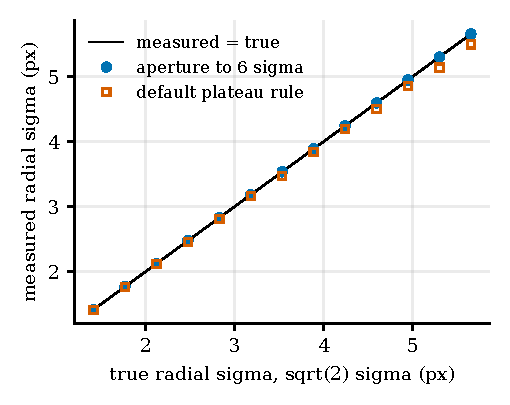
\includegraphics{build/fig_radial_sigma.pdf}\\
{\small Measured against true radial sigma, round Gaussian spots.}
\end{center}
\begin{longtable}{@{}p{0.86\textwidth}r@{}}
\toprule
test & result \\
\midrule
\endhead
radial sigma of a round gaussian is sqrt2 sigma\newline{\small\itshape sqrt(\textless{}r\textasciicircum{}2\textgreater{}) = sqrt(2) sigma in 2-D. Aperture out to 6 sigma; tolerance 1e-3.} & passed (3/3) \\
radial sigma does not depend on the brightness\newline{\small\itshape radial\_sigma(k A) = radial\_sigma(A); tolerance 1e-5.} & passed (3/3) \\
the default aperture cuts radial sigma by at most 5 percent\newline{\small\itshape With the plateau rule (R = 3.3 to 4 sigma): 0.95 sqrt(2) sigma \textless{} sqrt(\textless{}r\textasciicircum{}2\textgreater{}) \textless{} sqrt(2) sigma.} & passed (3/3) \\
\bottomrule
\end{longtable}

\section{Concentration}
$C = \sum_{r \le 2\,\mathrm{px}} w / \sum w$. For a continuous Gaussian $C = 1 - e^{-4/(2\sigma^2)}$.

\begin{center}
\begin{tabular}{lrrrrl}
\toprule
case & true & measured & relative error & tolerance & \\
\midrule
sigma = 1.5 px & 0.588888 & 0.602565 & $2.3\times10^{-2}$ & $5.0\times10^{-2}$ & ok \\
sigma = 2 px & 0.393469 & 0.404449 & $2.8\times10^{-2}$ & $5.0\times10^{-2}$ & ok \\
sigma = 3 px & 0.199263 & 0.20554 & $3.2\times10^{-2}$ & $5.0\times10^{-2}$ & ok \\
\bottomrule
\end{tabular}
\end{center}
\noindent{\small Against the continuous formula (spot centred 0.3, 0.2 px off a pixel).}

\begin{center}
\begin{tabular}{lrrrrl}
\toprule
case & true & measured & relative error & tolerance & \\
\midrule
sigma = 1.5 px & 0.602565 & 0.602565 & $1.1\times10^{-7}$ & $1.0\times10^{-4}$ & ok \\
sigma = 2 px & 0.404449 & 0.404449 & $1.1\times10^{-7}$ & $1.0\times10^{-4}$ & ok \\
sigma = 3 px & 0.20554 & 0.20554 & $6.8\times10^{-8}$ & $1.0\times10^{-4}$ & ok \\
\bottomrule
\end{tabular}
\end{center}
\noindent{\small Against the sum over the same pixels.}

\begin{center}
\begin{tabular}{lrrrrl}
\toprule
case & true & measured & relative error & tolerance & \\
\midrule
sigma = 1.5 px & 0.595036 & 0.536875 & $9.8\times10^{-2}$ & $1.5\times10^{-1}$ & ok \\
sigma = 2 px & 0.400725 & 0.352459 & $1.2\times10^{-1}$ & $1.5\times10^{-1}$ & ok \\
sigma = 3 px & 0.204534 & 0.176214 & $1.4\times10^{-1}$ & $1.5\times10^{-1}$ & ok \\
\bottomrule
\end{tabular}
\end{center}
\noindent{\small Spot centred exactly on a pixel: four pixels lie at exactly $r = 2$ and rounding decides which count.}

\begin{longtable}{@{}p{0.86\textwidth}r@{}}
\toprule
test & result \\
\midrule
\endhead
concentration of a gaussian is 1 minus exp\newline{\small\itshape C = 1 - exp(-4 / (2 sigma\textasciicircum{}2)). Tolerance 5 \%: whole pixels, not a disc.} & passed (3/3) \\
concentration equals the sum over the pixels within 2px\newline{\small\itshape C = sum over pixels with r \textless{}= 2 of exp(-r\textasciicircum{}2 / 2 sigma\textasciicircum{}2) / (2 pi sigma\textasciicircum{}2); tolerance 1e-4.} & passed (3/3) \\
concentration of a spot centred on a pixel is within 15 percent\newline{\small\itshape Same sum with the centre on a pixel: four pixels lie at exactly r = 2 and rounding decides; tolerance 15 \%.} & passed (3/3) \\
a narrower spot is more concentrated\newline{\small\itshape C decreases with sigma.} & passed \\
\bottomrule
\end{longtable}

\section{Eccentricity}
From the second moments of $w$ about the centroid, with eigenvalues $\lambda_1 \ge \lambda_2$: $e = \sqrt{1 - \lambda_2/\lambda_1}$. For an elliptical Gaussian $e = \sqrt{1 - \sigma_y^2/\sigma_x^2}$.

\begin{center}
\begin{tabular}{lrrrrl}
\toprule
case & true & measured & absolute error & tolerance & \\
\midrule
round, sigma = 1.5 px & 0 & 0 & 0 & $1.0\times10^{-2}$ & ok \\
round, sigma = 2 px & 0 & 0 & 0 & $1.0\times10^{-2}$ & ok \\
round, sigma = 3 px & 0 & 0 & 0 & $1.0\times10^{-2}$ & ok \\
sigma\_x = 3, sigma\_y = 2 px & 0.745356 & 0.745356 & $5.7\times10^{-8}$ & $1.0\times10^{-3}$ & ok \\
sigma\_x = 3, sigma\_y = 1.5 px & 0.866025 & 0.866025 & $2.1\times10^{-8}$ & $1.0\times10^{-3}$ & ok \\
sigma\_x = 4, sigma\_y = 2 px & 0.866025 & 0.866025 & $1.9\times10^{-8}$ & $1.0\times10^{-3}$ & ok \\
\bottomrule
\end{tabular}
\end{center}
\noindent{\small Along the pixel axes.}

\begin{center}
\begin{tabular}{lrrrrl}
\toprule
case & true & measured & relative error & tolerance & \\
\midrule
sigma\_x = 3, sigma\_y = 2 px, at 45 deg & 0.745356 & 0.745356 & $3.5\times10^{-8}$ & $1.0\times10^{-3}$ & ok \\
sigma\_x = 3, sigma\_y = 1.5 px, at 45 deg & 0.866025 & 0.866025 & $1.3\times10^{-8}$ & $1.0\times10^{-3}$ & ok \\
sigma\_x = 4, sigma\_y = 2 px, at 45 deg & 0.866025 & 0.866025 & $1.9\times10^{-8}$ & $1.0\times10^{-3}$ & ok \\
\bottomrule
\end{tabular}
\end{center}
\noindent{\small Turned by 45 degrees.}

\begin{center}
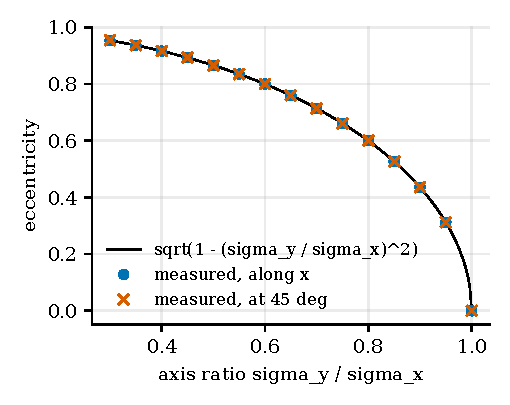
\includegraphics{build/fig_eccentricity.pdf}\\
{\small Eccentricity against the axis ratio, $\sigma_x = 4$ px.}
\end{center}
\begin{longtable}{@{}p{0.86\textwidth}r@{}}
\toprule
test & result \\
\midrule
\endhead
eccentricity of an elliptical gaussian\newline{\small\itshape e = sqrt(1 - sigma\_y\textasciicircum{}2 / sigma\_x\textasciicircum{}2); 0 for a round spot. Tolerance 1e-3 (0.01 absolute at e = 0).} & passed (6/6) \\
eccentricity does not change when the spot is turned by 45 degrees\newline{\small\itshape e(rotated by 45 deg) = sqrt(1 - sigma\_y\textasciicircum{}2 / sigma\_x\textasciicircum{}2); tolerance 1e-3.} & passed (3/3) \\
round spots have low eccentricity & passed \\
\bottomrule
\end{longtable}

\section{Profile slope}
The slope of the straight line fitted to $\ln w$ against $r$ over the aperture pixels with $w > 0$.

\begin{center}
\begin{tabular}{rr}
\toprule
$\sigma$ (px) & profile slope (1/px) \\
\midrule
1.5 & -1.595 \\
2 & -1.031 \\
3 & -0.67 \\
\bottomrule
\end{tabular}
\end{center}
\begin{longtable}{@{}p{0.86\textwidth}r@{}}
\toprule
test & result \\
\midrule
\endhead
profile slope is negative\newline{\small\itshape The light falls with distance: slope \textless{} 0.} & passed \\
profile slope is steeper for a narrower spot\newline{\small\itshape slope(sigma) increases towards 0 with sigma: more negative for a smaller sigma.} & passed \\
profile slope of an exponential spot is minus one over its length\newline{\small\itshape w = A exp(-r / L) -\textgreater{} log w = log A - r / L, slope = -1 / L; tolerance 1e-3.} & passed \\
fewer than three lit pixels give a slope of zero & passed \\
\bottomrule
\end{longtable}

\section{Isolation}
$d_i = \min_{j \ne i} |\mathbf{p}_i - \mathbf{p}_j|$; a spot is isolated when $d_i > f_{\mathrm{iso}}\,R_i$.

\begin{longtable}{@{}p{0.86\textwidth}r@{}}
\toprule
test & result \\
\midrule
\endhead
two spots at distance d have nn dist d\newline{\small\itshape nn\_dist = d for two spots d px apart (exact).} & passed (3/3) \\
nn dist is the distance to the nearest of several\newline{\small\itshape nn\_dist\_i = min over j != i of \textbar{}p\_i - p\_j\textbar{}: 3-4-5 triangle.} & passed \\
a single spot has infinite nn dist and is isolated\newline{\small\itshape One spot: nn\_dist = inf, is\_isolated = True.} & passed \\
is isolated flips exactly at factor times radius\newline{\small\itshape is\_isolated = nn\_dist \textgreater{} isolation\_factor * radius\_used (strictly).} & passed (4/4) \\
is isolated in an image follows the measured radius\newline{\small\itshape Two sigma = 1.5 spots (radius 6): crowded at 12 px, isolated at 13 px.} & passed \\
\bottomrule
\end{longtable}

\section{Brightness independence}
Concentration, eccentricity and profile slope are ratios of sums of $w$: $f(kA) = f(A)$.

\begin{center}
\begin{tabular}{lrrrrl}
\toprule
case & true & measured & relative error & tolerance & \\
\midrule
concentration, amplitude x 3 & 0.252545 & 0.252545 & $1.2\times10^{-7}$ & $1.0\times10^{-4}$ & ok \\
eccentricity, amplitude x 3 & 0.721348 & 0.721348 & $4.2\times10^{-9}$ & $1.0\times10^{-4}$ & ok \\
profile slope, amplitude x 3 & -0.857394 & -0.857395 & $8.4\times10^{-7}$ & $1.0\times10^{-4}$ & ok \\
\bottomrule
\end{tabular}
\end{center}
\noindent{\small The same spot, three times brighter.}

\begin{longtable}{@{}p{0.86\textwidth}r@{}}
\toprule
test & result \\
\midrule
\endhead
shape features do not change when the spot is 3 times brighter\newline{\small\itshape f(3 A) = f(A) for concentration, eccentricity, profile slope; tolerance 1e-4.} & passed (3/3) \\
shape features do not change when the spot is 4 times fainter\newline{\small\itshape f(A / 4) = f(A) for concentration, eccentricity, profile slope; tolerance 1e-4.} & passed (3/3) \\
\bottomrule
\end{longtable}

\section{Image luminosity and the count from light}
$L_{\mathrm{int}} = \sum_{\mathrm{MCP}} D - \bar b\,N_{\mathrm{MCP}}$, $\bar b$ the mean of the spot-free pixels; $N_{\mathrm{lum}} = L_{\mathrm{int}} / \langle L_{\mathrm{ap}} \rangle$, the mean light in a fixed aperture on the counted spots.

\begin{longtable}{@{}p{0.86\textwidth}r@{}}
\toprule
test & result \\
\midrule
\endhead
integrated light is the sum of the spots\newline{\small\itshape Three spots of 2 pi A sigma\textasciicircum{}2 each inside the circle -\textgreater{} 3 x that.} & passed \\
the count from light is the number of equal spots\newline{\small\itshape count = integrated light / mean aperture light per spot.} & passed \\
a flat residual floor is removed from the light\newline{\small\itshape The mean of the spot-free pixels is subtracted per pixel, so a floor of 0.7 counts changes nothing.} & passed \\
light outside the mcp circle is not integrated\newline{\small\itshape One spot inside the circle and one outside: only the first counts.} & passed \\
no spots gives a count of zero & passed \\
\bottomrule
\end{longtable}

\section{Separation score and best cut}
$s = |\mu_a - \mu_b| / (\sigma_a + \sigma_b)$. The best cut $t$ minimises $\frac{1}{2}[P(a > t) + P(b \le t)]$.

\begin{longtable}{@{}p{0.86\textwidth}r@{}}
\toprule
test & result \\
\midrule
\endhead
separation and best cut & passed \\
separation score is the mean difference over the summed widths\newline{\small\itshape score = \textbar{}mean\_a - mean\_b\textbar{} / (std\_a + std\_b): means 0 and 6, std 1 and 2 -\textgreater{} 2.} & passed \\
identical populations have a score of zero & passed \\
the best cut between two equal gaussians is half way\newline{\small\itshape Equal widths: the cut that minimises the error is (mean\_a + mean\_b) / 2, and each error is Phi(-d / 2 sigma).} & passed \\
disjoint populations are cut without error & passed \\
\bottomrule
\end{longtable}

\section{Principal components}
Columns standardised to $Z$, then $Z = U S V^{T}$: scores $US$, explained variance $S_k^2/\sum S^2$, loadings $V^{T}$. The ellipse is the $n\sigma$ contour of the covariance of two scores.

\begin{longtable}{@{}p{0.86\textwidth}r@{}}
\toprule
test & result \\
\midrule
\endhead
pca finds the direction of variance & passed \\
pca of two fully correlated columns has one component\newline{\small\itshape y = 3x: explained variance (1, 0), loading (1, 1) / sqrt(2).} & passed \\
pca scores are uncorrelated and carry the variance\newline{\small\itshape Columns are standardised first: total variance of the scores = number of columns.} & passed \\
a constant column does not break pca & passed \\
spot matrix keeps isolated finite spots only & passed \\
spot matrix takes log10 of the log features & passed \\
spot matrix of nothing has the right shape & passed \\
the ellipse is the n sigma contour of the covariance\newline{\small\itshape Points on a circle of radius 1: covariance = I n / (2 (n - 1)), so the 2 sigma ellipse is a circle of radius 2 sqrt(n / (2 (n - 1))).} & passed \\
the ellipse needs five points & passed \\
\bottomrule
\end{longtable}

\section{Run results}
\begin{longtable}{@{}p{0.86\textwidth}r@{}}
\toprule
test & result \\
\midrule
\endhead
analyse reports a bad image instead of raising & passed \\
analyse is detect with photometry plus the batman & passed \\
every run metric is a number & passed \\
metric falls back to pickup then batman then nan & passed \\
\bottomrule
\end{longtable}

\section{Averages and fits}
Repeats at the same $x$: mean and $s/\sqrt{n}$ (or $s$). Fits: $ax + b$, $ax^2 + bx + c$, $a\,e^{bx} + c$, with $R^2 = 1 - \sum (y - \hat y)^2 / \sum (y - \bar y)^2$.

\begin{longtable}{@{}p{0.86\textwidth}r@{}}
\toprule
test & result \\
\midrule
\endhead
averaging groups repeats & passed \\
the error is the standard error or the standard deviation\newline{\small\itshape sem = std(ddof=1) / sqrt(n); [10, 12, 14] -\textgreater{} std 2, sem 2 / sqrt(3).} & passed \\
a single run has no error bar & passed \\
averaging drops non finite points and sorts by x & passed \\
bin width groups nearby x and min n drops thin groups & passed \\
quadratic fit recovers its coefficients & passed \\
linear fit recovers slope and offset\newline{\small\itshape y = 3 x - 1 -\textgreater{} a = 3, b = -1, R\textasciicircum{}2 = 1.} & passed \\
exponential fit recovers its coefficients\newline{\small\itshape y = 40 exp(-0.5 x) + 5.} & passed \\
a weighted fit follows the precise points\newline{\small\itshape Two lines mixed: the points with small errors decide the fit.} & passed \\
an unknown model gives no fit & passed \\
\bottomrule
\end{longtable}

\section{Export and master archive}
\begin{longtable}{@{}p{0.86\textwidth}r@{}}
\toprule
test & result \\
\midrule
\endhead
export and master archive & passed \\
spots csv has one row per spot with the measured values & passed \\
failed runs are left out and progress is reported & passed \\
pickup columns are written next to the counts & passed \\
the master header grows and old rows keep their values & passed \\
\bottomrule
\end{longtable}

\section{Pickup: RF notch}
An IIR notch at $k f_0$ ($f_0 = 26.92$ MHz, $k = 1, 2, \dots$ below the Nyquist frequency), run forwards and backwards so the phase is zero and the pulse stays where it is.

\begin{center}
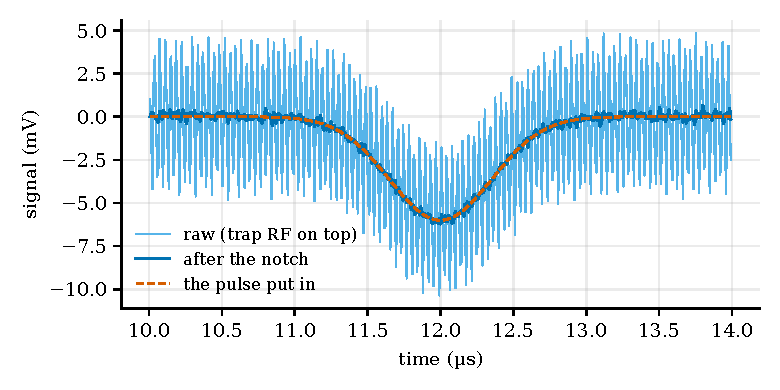
\includegraphics{build/fig_notch.pdf}\\
{\small A 6 mV pulse under 4 mV of trap RF, before and after the notch.}
\end{center}
\begin{longtable}{@{}p{0.86\textwidth}r@{}}
\toprule
test & result \\
\midrule
\endhead
notch skips frequencies above nyquist & passed \\
the fundamental and its harmonic are notched\newline{\small\itshape 4 mV at 26.92 MHz and 1.2 mV at 53.84 MHz: both below 1 \% after the notch.} & passed \\
harmonics at or above nyquist are left out\newline{\small\itshape At 125 MS/s: 26.92 and 53.84 MHz are notched, 80.76 MHz would alias.} & passed \\
one harmonic leaves the second alone & passed \\
a frequency away from the notch passes\newline{\small\itshape A 5 MHz signal keeps its amplitude within 1 \%.} & passed \\
the notch is zero phase the pulse does not move\newline{\small\itshape filtfilt runs the filter forwards and backwards: the peak of a 0.35 $\mu$s pulse stays within one sample (8 ns), with and without RF on top.} & passed (3/3) \\
the notch keeps the size of the pulse\newline{\small\itshape A 0.35 $\mu$s pulse has almost nothing at 27 MHz: amplitude and area within 2 \%.} & passed \\
the input trace is not modified & passed \\
\bottomrule
\end{longtable}

\section{Pickup: the pulse}
Baseline: median of the first 10\,\% of the trace; noise $1.4826\,\mathrm{MAD}$ there. The pulse is found when peak/noise $\ge n_\sigma$. Width: full width at half maximum. Area: $\sum (v - \mathrm{baseline})\,\Delta t$ while above $3\times$ noise.

\begin{longtable}{@{}p{0.86\textwidth}r@{}}
\toprule
test & result \\
\midrule
\endhead
a flat trace has no pulse & passed \\
a gaussian pulse is measured\newline{\small\itshape Amplitude A, time t0, FWHM = 2 sqrt(2 ln 2) w, area = A w sqrt(2 pi).} & passed (2/2) \\
the significance is the peak over the baseline noise\newline{\small\itshape n\_sigma = peak / (1.4826 MAD of the first 10 \% of the trace).} & passed \\
a pulse below the threshold is not found & passed \\
rf notch recovers a pulse buried in rf & passed \\
scope b is shifted by its batman delay & passed \\
scopes are found from filenames when tags do not match & passed \\
a folder without picoscope files gives nothing & passed \\
the notch is applied only to the chosen channels & passed \\
the columns are flat and named by scope and channel & passed \\
files are grouped by scope tag and channel & passed \\
a trace file gives its time axis in microseconds\newline{\small\itshape t = t0 + i dt with t0 = -10 $\mu$s, dt = 0.008 $\mu$s, 6000 samples.} & passed \\
\bottomrule
\end{longtable}

\section{Graphical interface}
\begin{longtable}{@{}p{0.86\textwidth}r@{}}
\toprule
test & result \\
\midrule
\endhead
the window opens on the image page with six pages & passed \\
each page is selected from the top bar & passed \\
each page is selected with ctrl and its number & passed \\
without data every page says what to do & passed \\
with data every page shows it & passed \\
the about window shows what about py says & passed \\
the shortcuts window lists the keys & passed \\
the top bar shows the version & passed \\
there is no separate menu bar & passed \\
file and help sit on the line of the tabs & passed \\
the menus hold every action & passed \\
every menu action does its job & passed \\
the shortcuts still trigger & passed \\
ctrl q closes the window & passed \\
every combo box has a label above it & passed \\
the combo labels look like the other small headings & passed \\
the style sheet points at arrow images that exist & passed \\
a combo box is drawn with a visible arrow & passed \\
the arrow turns phosphor green when the box has the focus & passed \\
a folder of runs becomes a dataset and its first run is shown & passed \\
each dataset gets its own colour and marker & passed \\
adding the same folder twice gives a second name & passed \\
loose images are added one item per file & passed \\
an empty folder adds nothing and says so & passed \\
clicking a run in the list makes it current & passed \\
page down and page up step through the runs across datasets & passed \\
the filter hides the runs that do not match & passed \\
removing the current dataset clears the view & passed \\
the live count equals detect on the same frame & passed \\
moving a slider updates the live result & passed \\
the slider and its number box stay in step & passed \\
reset defaults puts the settings back & passed \\
a frame that cannot be read shows an error not a count & passed \\
run all gives the same counts as analyse & passed \\
run all also measures the pickup of each run & passed \\
the button reads run all again after the settings change & passed \\
ctrl r runs all & passed \\
export writes files that agree with the session & passed \\
export uses the counted results not the current sliders & passed \\
export appends to the master archive & passed \\
a cancelled export writes nothing & passed \\
export before run all does nothing & passed \\
the export dialog remembers its folder & passed \\
the pickup page shows both scopes of the run & passed \\
one channel view draws the chosen trace & passed \\
switching the notch off loses the pulse & passed \\
a run without picoscope files says so & passed \\
apply to all counted runs fills the pickup columns & passed \\
find in files reads the scope tags from the filenames & passed \\
run all and export progress arrive on the gui thread & passed \\
\bottomrule
\end{longtable}

\section{Whole program}
\begin{longtable}{@{}p{0.86\textwidth}r@{}}
\toprule
test & result \\
\midrule
\endhead
reference frame matches golden & passed (6/6) \\
default params unchanged & passed \\
every public name is importable from the package & passed \\
importing the analysis does not import qt & passed \\
the cff reader finds the fields & passed \\
version agrees with citation cff and the package & passed \\
version agrees with pyproject & passed \\
release date agrees with citation cff & passed \\
title agrees with citation cff & passed \\
authors agree with citation cff & passed \\
licence agrees with citation cff & passed \\
doi agrees with citation cff & passed \\
the about lines carry every field & passed \\
the report contains every test name & passed \\
the report has its title version and sections & passed \\
the report gives true measured error and tolerance & passed \\
the report marks the tests it ran and those it did not & passed \\
the report figures are written & passed \\
the report does not touch the repository\newline{\small\itshape Everything goes to --out: a slip here once overwrote a test file.} & passed \\
the tex is well formed\newline{\small\itshape No LaTeX is run here; this catches the usual slips: an environment left open, unbalanced braces, an unescaped underscore in text.} & passed \\
\bottomrule
\end{longtable}

\section{All tests}
Every test by package, as pytest names it, with its result and the time it took.
\subsection*{Single-image analysis}
\begin{longtable}{@{}p{0.76\textwidth}lr@{}}
\toprule
test & result & time (s) \\
\midrule
\endhead
\path{tests/single_image_analysis/test_detection.py::test_finds_every_planted_spot} & passed & 0.02 \\
\path{tests/single_image_analysis/test_detection.py::test_empty_frame_has_no_spots} & passed & 0.01 \\
\path{tests/single_image_analysis/test_detection.py::test_raising_the_threshold_never_adds_spots} & passed & 0.02 \\
\path{tests/single_image_analysis/test_detection.py::test_photometry_does_not_change_the_count} & passed & 0.02 \\
\path{tests/single_image_analysis/test_detection.py::test_two_peaks_closer_than_min_dist_are_one_particle} & passed & 0.01 \\
\path{tests/single_image_analysis/test_detection.py::test_two_peaks_further_than_min_dist_are_two_particles} & passed & 0.01 \\
\path{tests/single_image_analysis/test_detection.py::test_a_flat_topped_spot_is_counted_once} & passed & 0.01 \\
\path{tests/single_image_analysis/test_detection.py::test_the_adaptive_threshold_is_the_larger_of_the_two} & passed & 0.01 \\
\path{tests/single_image_analysis/test_image_luminosity.py::test_integrated_light_is_the_sum_of_the_spots} & passed & 0.01 \\
\path{tests/single_image_analysis/test_image_luminosity.py::test_the_count_from_light_is_the_number_of_equal_spots} & passed & 0.01 \\
\path{tests/single_image_analysis/test_image_luminosity.py::test_a_flat_residual_floor_is_removed_from_the_light} & passed & 0.01 \\
\path{tests/single_image_analysis/test_image_luminosity.py::test_light_outside_the_mcp_circle_is_not_integrated} & passed & 0.00 \\
\path{tests/single_image_analysis/test_image_luminosity.py::test_no_spots_gives_a_count_of_zero} & passed & 0.00 \\
\path{tests/single_image_analysis/test_loading.py::test_scan_handles_run_folders_loose_images_and_files} & passed & 0.08 \\
\path{tests/single_image_analysis/test_loading.py::test_scan_of_a_single_run_folder_gives_one_item} & passed & 0.03 \\
\path{tests/single_image_analysis/test_loading.py::test_scan_of_nothing_useful_is_empty} & passed & 0.01 \\
\path{tests/single_image_analysis/test_loading.py::test_run_folders_are_sorted_by_run_number} & passed & 0.01 \\
\path{tests/single_image_analysis/test_loading.py::test_the_tiff_is_found_one_folder_down} & passed & 0.01 \\
\path{tests/single_image_analysis/test_loading.py::test_an_image_is_read_at_its_own_bit_depth} & passed & 0.01 \\
\path{tests/single_image_analysis/test_loading.py::test_batman_parameters_are_read} & passed & 0.02 \\
\path{tests/single_image_analysis/test_loading.py::test_a_missing_or_broken_batman_gives_no_parameters} & passed & 0.01 \\
\path{tests/single_image_analysis/test_preprocessing.py::test_hot_pixels_are_removed_not_counted} & passed & 0.01 \\
\path{tests/single_image_analysis/test_preprocessing.py::test_a_hot_pixel_is_replaced_by_its_3x3_median} & passed & 0.00 \\
\path{tests/single_image_analysis/test_preprocessing.py::test_hot_pixel_delta_zero_switches_the_correction_off} & passed & 0.00 \\
\path{tests/single_image_analysis/test_preprocessing.py::test_the_peak_of_a_real_spot_is_not_a_hot_pixel} & passed & 0.00 \\
\path{tests/single_image_analysis/test_preprocessing.py::test_hot_pixel_delta_scales_with_the_bit_depth} & passed & 0.00 \\
\path{tests/single_image_analysis/test_preprocessing.py::test_normalisation_is_by_bit_depth_not_content} & passed & 0.01 \\
\path{tests/single_image_analysis/test_preprocessing.py::test_the_full_scale_is_the_smallest_bit_depth_that_holds_the_maximum[200-255]} & passed & 0.00 \\
\path{tests/single_image_analysis/test_preprocessing.py::test_the_full_scale_is_the_smallest_bit_depth_that_holds_the_maximum[255-255]} & passed & 0.00 \\
\path{tests/single_image_analysis/test_preprocessing.py::test_the_full_scale_is_the_smallest_bit_depth_that_holds_the_maximum[256-1023]} & passed & 0.00 \\
\path{tests/single_image_analysis/test_preprocessing.py::test_the_full_scale_is_the_smallest_bit_depth_that_holds_the_maximum[1023-1023]} & passed & 0.00 \\
\path{tests/single_image_analysis/test_preprocessing.py::test_the_full_scale_is_the_smallest_bit_depth_that_holds_the_maximum[1024-4095]} & passed & 0.00 \\
\path{tests/single_image_analysis/test_preprocessing.py::test_the_full_scale_is_the_smallest_bit_depth_that_holds_the_maximum[4095-4095]} & passed & 0.00 \\
\path{tests/single_image_analysis/test_preprocessing.py::test_the_full_scale_is_the_smallest_bit_depth_that_holds_the_maximum[4096-65535]} & passed & 0.00 \\
\path{tests/single_image_analysis/test_preprocessing.py::test_the_full_scale_is_the_smallest_bit_depth_that_holds_the_maximum[65535-65535]} & passed & 0.00 \\
\path{tests/single_image_analysis/test_preprocessing.py::test_an_8_bit_image_is_not_rescaled} & passed & 0.00 \\
\path{tests/single_image_analysis/test_preprocessing.py::test_the_masked_background_does_not_rise_under_a_bright_spot} & passed & 0.01 \\
\path{tests/single_image_analysis/test_preprocessing.py::test_a_flat_image_has_itself_as_background} & passed & 0.00 \\
\path{tests/single_image_analysis/test_preprocessing.py::test_the_noise_estimate_is_the_gaussian_sigma} & passed & 0.03 \\
\path{tests/single_image_analysis/test_preprocessing.py::test_prepare_returns_a_non_negative_image_on_the_0_255_scale} & passed & 0.02 \\
\bottomrule
\end{longtable}
\subsection*{Spot features}
\begin{longtable}{@{}p{0.76\textwidth}lr@{}}
\toprule
test & result & time (s) \\
\midrule
\endhead
\path{tests/features/test_aperture.py::test_the_radius_grows_with_the_spot_size} & passed & 0.00 \\
\path{tests/features/test_aperture.py::test_the_radius_is_where_a_ring_adds_less_than_plateau_frac[sigma = 1.5 px]} & passed & 0.00 \\
\path{tests/features/test_aperture.py::test_the_radius_is_where_a_ring_adds_less_than_plateau_frac[sigma = 2 px]} & passed & 0.00 \\
\path{tests/features/test_aperture.py::test_the_radius_is_where_a_ring_adds_less_than_plateau_frac[sigma = 3 px]} & passed & 0.00 \\
\path{tests/features/test_aperture.py::test_the_radius_is_where_a_ring_adds_less_than_plateau_frac[sigma = 6 px]} & passed & 0.00 \\
\path{tests/features/test_aperture.py::test_the_radius_stops_at_spot_max_radius[5]} & passed & 0.00 \\
\path{tests/features/test_aperture.py::test_the_radius_stops_at_spot_max_radius[8]} & passed & 0.00 \\
\path{tests/features/test_aperture.py::test_the_radius_stops_at_spot_max_radius[12]} & passed & 0.00 \\
\path{tests/features/test_aperture.py::test_a_larger_plateau_frac_never_gives_a_larger_radius[1.5]} & passed & 0.00 \\
\path{tests/features/test_aperture.py::test_a_larger_plateau_frac_never_gives_a_larger_radius[2.0]} & passed & 0.00 \\
\path{tests/features/test_aperture.py::test_a_larger_plateau_frac_never_gives_a_larger_radius[3.0]} & passed & 0.00 \\
\path{tests/features/test_aperture.py::test_the_centroid_is_the_centre_of_the_spot} & passed & 0.00 \\
\path{tests/features/test_aperture.py::test_the_local_window_gives_the_same_numbers_as_the_full_frame} & passed & 0.00 \\
\path{tests/features/test_aperture.py::test_a_spot_at_the_image_edge_uses_the_pixels_that_exist} & passed & 0.00 \\
\path{tests/features/test_area.py::test_area_is_the_number_of_pixels_within_the_radius_used[sigma = 1.5 px, R = 6 px]} & passed & 0.00 \\
\path{tests/features/test_area.py::test_area_is_the_number_of_pixels_within_the_radius_used[sigma = 2 px, R = 7 px]} & passed & 0.00 \\
\path{tests/features/test_area.py::test_area_is_the_number_of_pixels_within_the_radius_used[sigma = 3 px, R = 10 px]} & passed & 0.00 \\
\path{tests/features/test_area.py::test_area_is_smaller_at_the_image_edge} & passed & 0.00 \\
\path{tests/features/test_brightness_independence.py::test_shape_features_do_not_change_when_the_spot_is_3_times_brighter[concentration, amplitude x 3]} & passed & 0.00 \\
\path{tests/features/test_brightness_independence.py::test_shape_features_do_not_change_when_the_spot_is_3_times_brighter[eccentricity, amplitude x 3]} & passed & 0.00 \\
\path{tests/features/test_brightness_independence.py::test_shape_features_do_not_change_when_the_spot_is_3_times_brighter[profile slope, amplitude x 3]} & passed & 0.00 \\
\path{tests/features/test_brightness_independence.py::test_shape_features_do_not_change_when_the_spot_is_4_times_fainter[concentration, amplitude x 0.25]} & passed & 0.00 \\
\path{tests/features/test_brightness_independence.py::test_shape_features_do_not_change_when_the_spot_is_4_times_fainter[eccentricity, amplitude x 0.25]} & passed & 0.00 \\
\path{tests/features/test_brightness_independence.py::test_shape_features_do_not_change_when_the_spot_is_4_times_fainter[profile slope, amplitude x 0.25]} & passed & 0.00 \\
\path{tests/features/test_concentration.py::test_concentration_of_a_gaussian_is_1_minus_exp[sigma = 1.5 px]} & passed & 0.00 \\
\path{tests/features/test_concentration.py::test_concentration_of_a_gaussian_is_1_minus_exp[sigma = 2 px]} & passed & 0.00 \\
\path{tests/features/test_concentration.py::test_concentration_of_a_gaussian_is_1_minus_exp[sigma = 3 px]} & passed & 0.00 \\
\path{tests/features/test_concentration.py::test_concentration_equals_the_sum_over_the_pixels_within_2px[sigma = 1.5 px]} & passed & 0.00 \\
\path{tests/features/test_concentration.py::test_concentration_equals_the_sum_over_the_pixels_within_2px[sigma = 2 px]} & passed & 0.00 \\
\path{tests/features/test_concentration.py::test_concentration_equals_the_sum_over_the_pixels_within_2px[sigma = 3 px]} & passed & 0.00 \\
\path{tests/features/test_concentration.py::test_concentration_of_a_spot_centred_on_a_pixel_is_within_15_percent[sigma = 1.5 px]} & passed & 0.00 \\
\path{tests/features/test_concentration.py::test_concentration_of_a_spot_centred_on_a_pixel_is_within_15_percent[sigma = 2 px]} & passed & 0.00 \\
\path{tests/features/test_concentration.py::test_concentration_of_a_spot_centred_on_a_pixel_is_within_15_percent[sigma = 3 px]} & passed & 0.00 \\
\path{tests/features/test_concentration.py::test_a_narrower_spot_is_more_concentrated} & passed & 0.00 \\
\path{tests/features/test_eccentricity.py::test_eccentricity_of_an_elliptical_gaussian[round, sigma = 1.5 px]} & passed & 0.00 \\
\path{tests/features/test_eccentricity.py::test_eccentricity_of_an_elliptical_gaussian[round, sigma = 2 px]} & passed & 0.00 \\
\path{tests/features/test_eccentricity.py::test_eccentricity_of_an_elliptical_gaussian[round, sigma = 3 px]} & passed & 0.00 \\
\path{tests/features/test_eccentricity.py::test_eccentricity_of_an_elliptical_gaussian[sigma_x = 3, sigma_y = 2 px]} & passed & 0.00 \\
\path{tests/features/test_eccentricity.py::test_eccentricity_of_an_elliptical_gaussian[sigma_x = 3, sigma_y = 1.5 px]} & passed & 0.00 \\
\path{tests/features/test_eccentricity.py::test_eccentricity_of_an_elliptical_gaussian[sigma_x = 4, sigma_y = 2 px]} & passed & 0.00 \\
\path{tests/features/test_eccentricity.py::test_eccentricity_does_not_change_when_the_spot_is_turned_by_45_degrees[sigma_x = 3, sigma_y = 2 px, at 45 deg]} & passed & 0.00 \\
\path{tests/features/test_eccentricity.py::test_eccentricity_does_not_change_when_the_spot_is_turned_by_45_degrees[sigma_x = 3, sigma_y = 1.5 px, at 45 deg]} & passed & 0.00 \\
\path{tests/features/test_eccentricity.py::test_eccentricity_does_not_change_when_the_spot_is_turned_by_45_degrees[sigma_x = 4, sigma_y = 2 px, at 45 deg]} & passed & 0.00 \\
\path{tests/features/test_eccentricity.py::test_round_spots_have_low_eccentricity} & passed & 0.01 \\
\path{tests/features/test_isolation.py::test_two_spots_at_distance_d_have_nn_dist_d[5]} & passed & 0.00 \\
\path{tests/features/test_isolation.py::test_two_spots_at_distance_d_have_nn_dist_d[13]} & passed & 0.00 \\
\path{tests/features/test_isolation.py::test_two_spots_at_distance_d_have_nn_dist_d[40]} & passed & 0.00 \\
\path{tests/features/test_isolation.py::test_nn_dist_is_the_distance_to_the_nearest_of_several} & passed & 0.00 \\
\path{tests/features/test_isolation.py::test_a_single_spot_has_infinite_nn_dist_and_is_isolated} & passed & 0.00 \\
\path{tests/features/test_isolation.py::test_is_isolated_flips_exactly_at_factor_times_radius[2.0-6]} & passed & 0.00 \\
\path{tests/features/test_isolation.py::test_is_isolated_flips_exactly_at_factor_times_radius[2.0-7]} & passed & 0.00 \\
\path{tests/features/test_isolation.py::test_is_isolated_flips_exactly_at_factor_times_radius[1.5-8]} & passed & 0.00 \\
\path{tests/features/test_isolation.py::test_is_isolated_flips_exactly_at_factor_times_radius[3.0-5]} & passed & 0.00 \\
\path{tests/features/test_isolation.py::test_is_isolated_in_an_image_follows_the_measured_radius} & passed & 0.00 \\
\path{tests/features/test_luminosity.py::test_luminosity_of_a_gaussian_is_2_pi_A_sigma_squared[sigma = 1.5 px]} & passed & 0.00 \\
\path{tests/features/test_luminosity.py::test_luminosity_of_a_gaussian_is_2_pi_A_sigma_squared[sigma = 2 px]} & passed & 0.00 \\
\path{tests/features/test_luminosity.py::test_luminosity_of_a_gaussian_is_2_pi_A_sigma_squared[sigma = 3 px]} & passed & 0.00 \\
\path{tests/features/test_luminosity.py::test_the_plateau_rule_keeps_the_luminosity_within_3_percent[sigma = 1.5 px, R = 6 px]} & passed & 0.00 \\
\path{tests/features/test_luminosity.py::test_the_plateau_rule_keeps_the_luminosity_within_3_percent[sigma = 2 px, R = 7 px]} & passed & 0.00 \\
\path{tests/features/test_luminosity.py::test_the_plateau_rule_keeps_the_luminosity_within_3_percent[sigma = 3 px, R = 10 px]} & passed & 0.00 \\
\path{tests/features/test_luminosity.py::test_doubling_the_amplitude_doubles_the_luminosity[1.5]} & passed & 0.00 \\
\path{tests/features/test_luminosity.py::test_doubling_the_amplitude_doubles_the_luminosity[2.0]} & passed & 0.00 \\
\path{tests/features/test_luminosity.py::test_doubling_the_amplitude_doubles_the_luminosity[3.0]} & passed & 0.00 \\
\path{tests/features/test_luminosity.py::test_luminosity_through_the_whole_pipeline_is_within_7_percent[sigma = 1.5 px, R = 6 px]} & passed & 0.00 \\
\path{tests/features/test_luminosity.py::test_luminosity_through_the_whole_pipeline_is_within_7_percent[sigma = 2 px, R = 7 px]} & passed & 0.00 \\
\path{tests/features/test_luminosity.py::test_luminosity_through_the_whole_pipeline_is_within_7_percent[sigma = 3 px, R = 9 px]} & passed & 0.00 \\
\path{tests/features/test_luminosity.py::test_a_flat_offset_does_not_change_the_luminosity[1.5]} & passed & 0.01 \\
\path{tests/features/test_luminosity.py::test_a_flat_offset_does_not_change_the_luminosity[2.0]} & passed & 0.01 \\
\path{tests/features/test_luminosity.py::test_a_flat_offset_does_not_change_the_luminosity[3.0]} & passed & 0.01 \\
\path{tests/features/test_luminosity.py::test_photometry_measures_brighter_spots_as_brighter} & passed & 0.03 \\
\path{tests/features/test_profile_slope.py::test_profile_slope_is_negative} & passed & 0.00 \\
\path{tests/features/test_profile_slope.py::test_profile_slope_is_steeper_for_a_narrower_spot} & passed & 0.00 \\
\path{tests/features/test_profile_slope.py::test_profile_slope_of_an_exponential_spot_is_minus_one_over_its_length} & passed & 0.00 \\
\path{tests/features/test_profile_slope.py::test_fewer_than_three_lit_pixels_give_a_slope_of_zero} & passed & 0.00 \\
\path{tests/features/test_radial_sigma.py::test_radial_sigma_of_a_round_gaussian_is_sqrt2_sigma[sigma = 1.5 px]} & passed & 0.00 \\
\path{tests/features/test_radial_sigma.py::test_radial_sigma_of_a_round_gaussian_is_sqrt2_sigma[sigma = 2 px]} & passed & 0.00 \\
\path{tests/features/test_radial_sigma.py::test_radial_sigma_of_a_round_gaussian_is_sqrt2_sigma[sigma = 3 px]} & passed & 0.00 \\
\path{tests/features/test_radial_sigma.py::test_radial_sigma_does_not_depend_on_the_brightness[1.5]} & passed & 0.00 \\
\path{tests/features/test_radial_sigma.py::test_radial_sigma_does_not_depend_on_the_brightness[2.0]} & passed & 0.00 \\
\path{tests/features/test_radial_sigma.py::test_radial_sigma_does_not_depend_on_the_brightness[3.0]} & passed & 0.00 \\
\path{tests/features/test_radial_sigma.py::test_the_default_aperture_cuts_radial_sigma_by_at_most_5_percent[1.5]} & passed & 0.00 \\
\path{tests/features/test_radial_sigma.py::test_the_default_aperture_cuts_radial_sigma_by_at_most_5_percent[2.0]} & passed & 0.00 \\
\path{tests/features/test_radial_sigma.py::test_the_default_aperture_cuts_radial_sigma_by_at_most_5_percent[3.0]} & passed & 0.00 \\
\bottomrule
\end{longtable}
\subsection*{Clustering and recognition}
\begin{longtable}{@{}p{0.76\textwidth}lr@{}}
\toprule
test & result & time (s) \\
\midrule
\endhead
\path{tests/clustering_recognition/test_pca.py::test_pca_finds_the_direction_of_variance} & passed & 0.63 \\
\path{tests/clustering_recognition/test_pca.py::test_pca_of_two_fully_correlated_columns_has_one_component} & passed & 0.00 \\
\path{tests/clustering_recognition/test_pca.py::test_pca_scores_are_uncorrelated_and_carry_the_variance} & passed & 0.00 \\
\path{tests/clustering_recognition/test_pca.py::test_a_constant_column_does_not_break_pca} & passed & 0.00 \\
\path{tests/clustering_recognition/test_pca.py::test_spot_matrix_keeps_isolated_finite_spots_only} & passed & 0.00 \\
\path{tests/clustering_recognition/test_pca.py::test_spot_matrix_takes_log10_of_the_log_features} & passed & 0.00 \\
\path{tests/clustering_recognition/test_pca.py::test_spot_matrix_of_nothing_has_the_right_shape} & passed & 0.00 \\
\path{tests/clustering_recognition/test_pca.py::test_the_ellipse_is_the_n_sigma_contour_of_the_covariance} & passed & 0.00 \\
\path{tests/clustering_recognition/test_pca.py::test_the_ellipse_needs_five_points} & passed & 0.00 \\
\path{tests/clustering_recognition/test_separation.py::test_separation_and_best_cut} & passed & 0.01 \\
\path{tests/clustering_recognition/test_separation.py::test_separation_score_is_the_mean_difference_over_the_summed_widths} & passed & 0.00 \\
\path{tests/clustering_recognition/test_separation.py::test_identical_populations_have_a_score_of_zero} & passed & 0.00 \\
\path{tests/clustering_recognition/test_separation.py::test_the_best_cut_between_two_equal_gaussians_is_half_way} & passed & 0.02 \\
\path{tests/clustering_recognition/test_separation.py::test_disjoint_populations_are_cut_without_error} & passed & 0.00 \\
\bottomrule
\end{longtable}
\subsection*{Results}
\begin{longtable}{@{}p{0.76\textwidth}lr@{}}
\toprule
test & result & time (s) \\
\midrule
\endhead
\path{tests/results/test_export.py::test_export_and_master_archive} & passed & 0.37 \\
\path{tests/results/test_export.py::test_spots_csv_has_one_row_per_spot_with_the_measured_values} & passed & 0.10 \\
\path{tests/results/test_export.py::test_failed_runs_are_left_out_and_progress_is_reported} & passed & 0.28 \\
\path{tests/results/test_export.py::test_pickup_columns_are_written_next_to_the_counts} & passed & 0.11 \\
\path{tests/results/test_export.py::test_the_master_header_grows_and_old_rows_keep_their_values} & passed & 0.13 \\
\path{tests/results/test_run.py::test_analyse_reports_a_bad_image_instead_of_raising} & passed & 0.00 \\
\path{tests/results/test_run.py::test_analyse_is_detect_with_photometry_plus_the_batman} & passed & 0.08 \\
\path{tests/results/test_run.py::test_every_run_metric_is_a_number} & passed & 0.05 \\
\path{tests/results/test_run.py::test_metric_falls_back_to_pickup_then_batman_then_nan} & passed & 0.00 \\
\path{tests/results/test_trends.py::test_averaging_groups_repeats} & passed & 0.00 \\
\path{tests/results/test_trends.py::test_the_error_is_the_standard_error_or_the_standard_deviation} & passed & 0.00 \\
\path{tests/results/test_trends.py::test_a_single_run_has_no_error_bar} & passed & 0.00 \\
\path{tests/results/test_trends.py::test_averaging_drops_non_finite_points_and_sorts_by_x} & passed & 0.00 \\
\path{tests/results/test_trends.py::test_bin_width_groups_nearby_x_and_min_n_drops_thin_groups} & passed & 0.00 \\
\path{tests/results/test_trends.py::test_quadratic_fit_recovers_its_coefficients} & passed & 0.00 \\
\path{tests/results/test_trends.py::test_linear_fit_recovers_slope_and_offset} & passed & 0.00 \\
\path{tests/results/test_trends.py::test_exponential_fit_recovers_its_coefficients} & passed & 0.00 \\
\path{tests/results/test_trends.py::test_a_weighted_fit_follows_the_precise_points} & passed & 0.00 \\
\path{tests/results/test_trends.py::test_an_unknown_model_gives_no_fit} & passed & 0.00 \\
\bottomrule
\end{longtable}
\subsection*{Pickup}
\begin{longtable}{@{}p{0.76\textwidth}lr@{}}
\toprule
test & result & time (s) \\
\midrule
\endhead
\path{tests/pickup/test_measure.py::test_rf_notch_recovers_a_pulse_buried_in_rf} & passed & 0.20 \\
\path{tests/pickup/test_measure.py::test_scope_b_is_shifted_by_its_batman_delay} & passed & 0.31 \\
\path{tests/pickup/test_measure.py::test_scopes_are_found_from_filenames_when_tags_do_not_match} & passed & 0.18 \\
\path{tests/pickup/test_measure.py::test_a_folder_without_picoscope_files_gives_nothing} & passed & 0.00 \\
\path{tests/pickup/test_measure.py::test_the_notch_is_applied_only_to_the_chosen_channels} & passed & 0.15 \\
\path{tests/pickup/test_measure.py::test_the_columns_are_flat_and_named_by_scope_and_channel} & passed & 0.15 \\
\path{tests/pickup/test_measure.py::test_files_are_grouped_by_scope_tag_and_channel} & passed & 0.04 \\
\path{tests/pickup/test_measure.py::test_a_trace_file_gives_its_time_axis_in_microseconds} & passed & 0.06 \\
\path{tests/pickup/test_pulse.py::test_a_flat_trace_has_no_pulse} & passed & 0.00 \\
\path{tests/pickup/test_pulse.py::test_a_gaussian_pulse_is_measured[1]} & passed & 0.00 \\
\path{tests/pickup/test_pulse.py::test_a_gaussian_pulse_is_measured[-1]} & passed & 0.00 \\
\path{tests/pickup/test_pulse.py::test_the_significance_is_the_peak_over_the_baseline_noise} & passed & 0.00 \\
\path{tests/pickup/test_pulse.py::test_a_pulse_below_the_threshold_is_not_found} & passed & 0.00 \\
\path{tests/pickup/test_rf_filter.py::test_notch_skips_frequencies_above_nyquist} & passed & 0.00 \\
\path{tests/pickup/test_rf_filter.py::test_the_fundamental_and_its_harmonic_are_notched} & passed & 0.00 \\
\path{tests/pickup/test_rf_filter.py::test_harmonics_at_or_above_nyquist_are_left_out} & passed & 0.00 \\
\path{tests/pickup/test_rf_filter.py::test_one_harmonic_leaves_the_second_alone} & passed & 0.00 \\
\path{tests/pickup/test_rf_filter.py::test_a_frequency_away_from_the_notch_passes} & passed & 0.00 \\
\path{tests/pickup/test_rf_filter.py::test_the_notch_is_zero_phase_the_pulse_does_not_move[12.0]} & passed & 0.00 \\
\path{tests/pickup/test_rf_filter.py::test_the_notch_is_zero_phase_the_pulse_does_not_move[20.004]} & passed & 0.00 \\
\path{tests/pickup/test_rf_filter.py::test_the_notch_is_zero_phase_the_pulse_does_not_move[31.5]} & passed & 0.00 \\
\path{tests/pickup/test_rf_filter.py::test_the_notch_keeps_the_size_of_the_pulse} & passed & 0.00 \\
\path{tests/pickup/test_rf_filter.py::test_the_input_trace_is_not_modified} & passed & 0.00 \\
\bottomrule
\end{longtable}
\subsection*{Graphical interface}
\begin{longtable}{@{}p{0.76\textwidth}lr@{}}
\toprule
test & result & time (s) \\
\midrule
\endhead
\path{tests/graphical_interface/test_combo_boxes.py::test_every_combo_box_has_a_label_above_it} & passed & 6.40 \\
\path{tests/graphical_interface/test_combo_boxes.py::test_the_combo_labels_look_like_the_other_small_headings} & passed & 0.55 \\
\path{tests/graphical_interface/test_combo_boxes.py::test_the_style_sheet_points_at_arrow_images_that_exist} & passed & 0.02 \\
\path{tests/graphical_interface/test_combo_boxes.py::test_a_combo_box_is_drawn_with_a_visible_arrow} & passed & 0.58 \\
\path{tests/graphical_interface/test_combo_boxes.py::test_the_arrow_turns_phosphor_green_when_the_box_has_the_focus} & passed & 0.69 \\
\path{tests/graphical_interface/test_datasets.py::test_a_folder_of_runs_becomes_a_dataset_and_its_first_run_is_shown} & passed & 7.23 \\
\path{tests/graphical_interface/test_datasets.py::test_each_dataset_gets_its_own_colour_and_marker} & passed & 0.75 \\
\path{tests/graphical_interface/test_datasets.py::test_adding_the_same_folder_twice_gives_a_second_name} & passed & 0.94 \\
\path{tests/graphical_interface/test_datasets.py::test_loose_images_are_added_one_item_per_file} & passed & 0.81 \\
\path{tests/graphical_interface/test_datasets.py::test_an_empty_folder_adds_nothing_and_says_so} & passed & 0.56 \\
\path{tests/graphical_interface/test_datasets.py::test_clicking_a_run_in_the_list_makes_it_current} & passed & 1.32 \\
\path{tests/graphical_interface/test_datasets.py::test_page_down_and_page_up_step_through_the_runs_across_datasets} & passed & 2.24 \\
\path{tests/graphical_interface/test_datasets.py::test_the_filter_hides_the_runs_that_do_not_match} & passed & 0.75 \\
\path{tests/graphical_interface/test_datasets.py::test_removing_the_current_dataset_clears_the_view} & passed & 0.86 \\
\path{tests/graphical_interface/test_live_detection.py::test_the_live_count_equals_detect_on_the_same_frame} & passed & 0.88 \\
\path{tests/graphical_interface/test_live_detection.py::test_moving_a_slider_updates_the_live_result} & passed & 2.84 \\
\path{tests/graphical_interface/test_live_detection.py::test_the_slider_and_its_number_box_stay_in_step} & passed & 0.58 \\
\path{tests/graphical_interface/test_live_detection.py::test_reset_defaults_puts_the_settings_back} & passed & 1.37 \\
\path{tests/graphical_interface/test_live_detection.py::test_a_frame_that_cannot_be_read_shows_an_error_not_a_count} & passed & 0.47 \\
\path{tests/graphical_interface/test_pickup_page.py::test_the_pickup_page_shows_both_scopes_of_the_run} & passed & 16.15 \\
\path{tests/graphical_interface/test_pickup_page.py::test_one_channel_view_draws_the_chosen_trace} & passed & 1.72 \\
\path{tests/graphical_interface/test_pickup_page.py::test_switching_the_notch_off_loses_the_pulse} & passed & 1.39 \\
\path{tests/graphical_interface/test_pickup_page.py::test_a_run_without_picoscope_files_says_so} & passed & 1.33 \\
\path{tests/graphical_interface/test_pickup_page.py::test_apply_to_all_counted_runs_fills_the_pickup_columns} & passed & 2.04 \\
\path{tests/graphical_interface/test_pickup_page.py::test_find_in_files_reads_the_scope_tags_from_the_filenames} & passed & 1.10 \\
\path{tests/graphical_interface/test_run_all_export.py::test_run_all_gives_the_same_counts_as_analyse} & passed & 2.46 \\
\path{tests/graphical_interface/test_run_all_export.py::test_run_all_also_measures_the_pickup_of_each_run} & passed & 1.36 \\
\path{tests/graphical_interface/test_run_all_export.py::test_the_button_reads_run_all_again_after_the_settings_change} & passed & 2.10 \\
\path{tests/graphical_interface/test_run_all_export.py::test_ctrl_r_runs_all} & passed & 1.36 \\
\path{tests/graphical_interface/test_run_all_export.py::test_export_writes_files_that_agree_with_the_session} & passed & 1.43 \\
\path{tests/graphical_interface/test_run_all_export.py::test_export_uses_the_counted_results_not_the_current_sliders} & passed & 1.72 \\
\path{tests/graphical_interface/test_run_all_export.py::test_export_appends_to_the_master_archive} & passed & 1.40 \\
\path{tests/graphical_interface/test_run_all_export.py::test_a_cancelled_export_writes_nothing} & passed & 1.25 \\
\path{tests/graphical_interface/test_run_all_export.py::test_export_before_run_all_does_nothing} & passed & 0.72 \\
\path{tests/graphical_interface/test_run_all_export.py::test_the_export_dialog_remembers_its_folder} & passed & 0.54 \\
\path{tests/graphical_interface/test_start.py::test_python_m_dipesh_starts_the_app_and_selftest_closes_it} & passed & 2.58 \\
\path{tests/graphical_interface/test_start.py::test_the_dipesh_entry_point_is_the_same_main} & passed & 0.00 \\
\path{tests/graphical_interface/test_threads.py::test_run_all_and_export_progress_arrive_on_the_gui_thread} & passed & 2.01 \\
\path{tests/graphical_interface/test_top_bar.py::test_there_is_no_separate_menu_bar} & passed & 0.55 \\
\path{tests/graphical_interface/test_top_bar.py::test_file_and_help_sit_on_the_line_of_the_tabs} & passed & 0.67 \\
\path{tests/graphical_interface/test_top_bar.py::test_the_menus_hold_every_action} & passed & 0.59 \\
\path{tests/graphical_interface/test_top_bar.py::test_every_menu_action_does_its_job} & passed & 1.45 \\
\path{tests/graphical_interface/test_top_bar.py::test_the_shortcuts_still_trigger} & passed & 2.44 \\
\path{tests/graphical_interface/test_top_bar.py::test_ctrl_q_closes_the_window} & passed & 0.52 \\
\path{tests/graphical_interface/test_window.py::test_the_window_opens_on_the_image_page_with_six_pages} & passed & 0.51 \\
\path{tests/graphical_interface/test_window.py::test_each_page_is_selected_from_the_top_bar} & passed & 0.67 \\
\path{tests/graphical_interface/test_window.py::test_each_page_is_selected_with_ctrl_and_its_number} & passed & 0.71 \\
\path{tests/graphical_interface/test_window.py::test_without_data_every_page_says_what_to_do} & passed & 0.87 \\
\path{tests/graphical_interface/test_window.py::test_with_data_every_page_shows_it} & passed & 1.87 \\
\path{tests/graphical_interface/test_window.py::test_the_about_window_shows_what_about_py_says} & passed & 0.49 \\
\path{tests/graphical_interface/test_window.py::test_the_shortcuts_window_lists_the_keys} & passed & 0.58 \\
\path{tests/graphical_interface/test_window.py::test_the_top_bar_shows_the_version} & passed & 0.53 \\
\bottomrule
\end{longtable}
\subsection*{Whole program}
\begin{longtable}{@{}p{0.76\textwidth}lr@{}}
\toprule
test & result & time (s) \\
\midrule
\endhead
\path{tests/test_about.py::test_the_cff_reader_finds_the_fields} & passed & 0.00 \\
\path{tests/test_about.py::test_version_agrees_with_citation_cff_and_the_package} & passed & 0.00 \\
\path{tests/test_about.py::test_version_agrees_with_pyproject} & passed & 0.00 \\
\path{tests/test_about.py::test_release_date_agrees_with_citation_cff} & passed & 0.00 \\
\path{tests/test_about.py::test_title_agrees_with_citation_cff} & passed & 0.00 \\
\path{tests/test_about.py::test_authors_agree_with_citation_cff} & passed & 0.00 \\
\path{tests/test_about.py::test_licence_agrees_with_citation_cff} & passed & 0.00 \\
\path{tests/test_about.py::test_doi_agrees_with_citation_cff} & passed & 0.00 \\
\path{tests/test_about.py::test_the_about_lines_carry_every_field} & passed & 0.00 \\
\path{tests/test_golden.py::test_reference_frame_matches_golden[frame_1.tiff]} & passed & 0.17 \\
\path{tests/test_golden.py::test_reference_frame_matches_golden[frame_2.tiff]} & passed & 0.24 \\
\path{tests/test_golden.py::test_reference_frame_matches_golden[frame_3.tiff]} & passed & 0.24 \\
\path{tests/test_golden.py::test_reference_frame_matches_golden[frame_4.tiff]} & passed & 0.24 \\
\path{tests/test_golden.py::test_reference_frame_matches_golden[frame_5.tiff]} & passed & 0.22 \\
\path{tests/test_golden.py::test_reference_frame_matches_golden[frame_6.tiff]} & passed & 0.22 \\
\path{tests/test_golden.py::test_default_params_unchanged} & passed & 0.00 \\
\path{tests/test_public_api.py::test_every_public_name_is_importable_from_the_package} & passed & 0.00 \\
\path{tests/test_public_api.py::test_importing_the_analysis_does_not_import_qt} & passed & 0.22 \\
\path{tests/test_report.py::test_the_report_contains_every_test_name} & passed & 10.24 \\
\path{tests/test_report.py::test_the_report_has_its_title_version_and_sections} & passed & 0.00 \\
\path{tests/test_report.py::test_the_report_gives_true_measured_error_and_tolerance} & passed & 0.00 \\
\path{tests/test_report.py::test_the_report_marks_the_tests_it_ran_and_those_it_did_not} & passed & 0.00 \\
\path{tests/test_report.py::test_the_report_figures_are_written} & passed & 0.00 \\
\path{tests/test_report.py::test_the_report_does_not_touch_the_repository} & passed & 0.00 \\
\path{tests/test_report.py::test_the_tex_is_well_formed} & passed & 0.01 \\
\bottomrule
\end{longtable}
\end{document}
